%----------------------------------------------------------------
%
%  File    :  vpn_prelim.tex
%
%  Author  :  Keith Andrews, IICM, TU Graz, Austria
% 
%  Created :  22 Feb 96
% 
%  Changed :  19 Feb 2004
% 
%----------------------------------------------------------------

\chapter{Preliminaries}

\label{chap:Preliminaries}

\iffalse
\section{Deterministic Finite Automata}
A \ac{dfa} is a finite-state machine that is defined as a quintuple $D = \{S, s_0, \Sigma, \delta, F\}$ where $S$ is a finite set of states, $s_0 \in S$ is the initial state, $\Sigma$ is a finite set called the input alphabet, $\delta$ is the state-transition function $\delta \colon S \times \Sigma \rightarrow S$ that maps a state and an element of the input alphabet to another state in $S$ and $F$ is the set of accepting states. \Acp{dfa} do not have any output.
\fi

\section{Mealy Machines}
Mealy machines are a modeling formalism for reactive systems such as communication protocols. Mealy machines are finite-state machines in which each transition is labeled with an input and a corresponding output action. More formally, a Mealy machine is defined as a 6-tuple $M = \{S, s_0, \Sigma, O, \delta, \lambda\}$, where $S$ is a finite set of states, $s_0 \in S$ is the initial state, $\Sigma$ is a finite set called the input alphabet, $O$ is a finite set called the output alphabet, $\delta$ is the state-transition function $\delta \colon S \times \Sigma \rightarrow S$ that maps a state and an element of the input alphabet to another state in $S$. In other words, the choice of each new state is defined by the current state and an external input. Finally, $\lambda$ is the output function $\lambda \colon S \times \Sigma \rightarrow O$ which maps a state-input alphabet pair to an element of the output alphabet $O$. We use Mealy machines to model the state of learned \ac{ipsec} implementations.

\section{Automata Learning}
Automata learning refers to methods of learning a behavioral model of a system through an algorithm or process. The learned model describes the behavior of the \ac{sul}. We differentiate between active and passive automata learning. In passive automata learning, models are learned based on a given data set describing the behavior of the \ac{sul}, e.g. log files. In contrast, in \acf{aal} the \ac{sul} is queried directly. In this paper, we will focus on \ac{aal} and will, moving on, be referring to it as automata learning or \ac{aal} interchangeably. 

One of the most influential AAL algorithms was introduced in 1987 by Dana Angluin, titled ``Learning regular sets from queries and counterexamples''~\cite{ANGLUIN198787}. In this seminal paper, Angluin introduced the concept of the \ac{mat} as well as an algorithm for learning regular languages from queries and counterexamples, called $L^*$. Note, that while the $L^*$ algorithm was originally designed to learn \acp{dfa} of regular languages, it can be simply extended to work for Mealy machines by making use of the similarities between \acp{dfa} and Mealy machines~\cite{hungar2003domain, shahbaz2009inferring}. As Mealy machines are our chosen formalism for modeling learned reactive systems, we will assume throughout this paper that we employ the Mealy machine variants of all mentioned learning algorithms. 

\iffalse
$L^*$ uses the \ac{mat} framework to learn an unknown regular language $L$. The \ac{mat} framework defines both a learner and a teacher. The teacher must respond to two types of queries posed by the learner, namely membership and equivalence queries. Queries are built using a fixed input alphabet $\Sigma$ where $L \subseteq \Sigma^*$ must hold. Membership queries consist of a word $s \in \Sigma^*$ and must be answered with either ``yes'' if $s \in L$, or ``no'' if not. In other words, membership queries are used to check if a given word is part of the language being learned. The learner proposes a regular language $L\mathrm{prop}$ and sends it to the teacher as an equivalence query. The teacher must confirm if $L\mathrm{prop}$ is equivalent to $L$, answering with  ``yes'' if the equivalence holds true, or else returning a counterexample $c$ proving the two languages are different. In other words, equivalence queries are used to verify if the learner has successfully learned the target language $L$ or if not, return a counterexample detailing the differences.
\fi

\subsection{MAT Framework}

$L^*$ uses the \ac{mat} framework to learn a Mealy machine representation of the behavior of an unknown system. To this end, the \ac{mat} framework defines both a learner and a teacher. The teacher must respond to two types of queries posed by the learner, namely output and equivalence queries. Note that in the original $L^*$ paper, the term membership query is used instead of output queries. The term output queries is used when learning Mealy machines. On a conceptual level, the learner poses output queries to the teacher in order to build a behavioral model of the \ac{sul} and equivalence queries, to verify if the model accurately describes the behavior of the system. Output queries consist of an input $s \in \Sigma^*$, where $\Sigma$ is the input alphabet. The teacher receives the output query and executes it on the \ac{sul}, returning the response of the \ac{sul} to the learner. In other words, using the Mealy machine definition from before, output queries are used to learn the mapping between inputs $s \in \Sigma^*$ to an outputs $o \in O$. Once enough information has been gathered using output queries, the learner constructs a Mealy machine representation of the \ac{sul} and proposes it to the teacher as an equivalence query. The teacher must confirm if the proposal is equivalent to the \ac{sul}, answering with  ``yes'' if the equivalence holds true, or else returning a counterexample that represents an input sequence that reveals the behavioral difference between the provided model and the \ac{sul}, proving their non-equivalence. In other words, equivalence queries are used to verify if the learner has successfully learned the Mealy machine representation of the \ac{sul} or if not, return a counterexample detailing the differences. If a counterexample is returned by the teacher, the learner uses this to update its model to include the new information and starts the cycle anew. This cycle of repeatedly gathering information through output queries and proposing a model through an equivalence query until it is confirmed to be correct is showcased in Figure~\ref{fig:mat} below. We can see that the algorithm does not end until the teacher confirms that the proposed model is equivalent.

\iffalse
\TODO{rework as control-flow diagram}
\begin{lstlisting}[mathescape=true, float=ht, caption=MAT algorithm, label=lst:mat]
	$\mathbf{Initialization}$
	
	$\mathbf{repeat}$:
		Output query
		
		$\mathbf{if}$: Sufficient information has been gathered through output queries
			Construct Mealy Machine proposal $L\mathrm{prop}$.
			Equivalence query($L\mathrm{prop}$)
			
			$\mathbf{if}$: Query returns "yes" $\mathbf{then}$
				$\mathbf{return}$ $L\mathrm{prop}$
			$\mathbf{else}$:
				Parse counterexample
			$\mathbf{fi}$
		$\mathbf{fi}$
	$\mathbf{end}$
	
\end{lstlisting}
\fi

\begin{figure}
	\centering
	\begin{tikzpicture}[->]
		% Draw the vertices.
		\node at (0,0) [rectangle, draw, fill=lightgray, minimum width=4cm, minimum height=1.2cm] (i) {Initial State};
		\node[rectangle, draw, fill=lightgray, minimum height=1.2cm, below of=i, node distance=1.8cm, minimum width=4cm] (s) {Output Queries};
		\node[diamond, draw, aspect=2, below of=s, node distance=1.8cm, scale=0.7] (a) {Construct Hypothesis};
		\node[rectangle, draw, below of=a, node distance=1.8cm, fill=lightgray, minimum height=1.2cm, minimum width=4cm] (b) {Equivalence Query};
		\node[diamond, draw, aspect=2, below of=b, node distance=2cm, scale=0.7] (c) {Teacher Response};
		\node[rectangle, draw, below of=c, node distance=2cm, fill=lightgray, minimum height=1.2cm, minimum width=4cm] (d) {Return Learned Model};
		
		% Connect vertices with edges
		\path (i) edge node {} (s);
		\path (s) edge node {} (a);
		\path (a) edge node {} (b);
		\path (b) edge node {} (c);
		\path (c) edge node [right] {yes} (d);
		\path (c) edge [out=0,in=0,looseness=1] node [right] {no} (s);
	\end{tikzpicture}
	\label{fig:mat}
\end{figure}


\subsection{L\textsuperscript{*}}
$L^*$ uses the \ac{mat} framework and stores the results of the output queries in a data structure called the observation table. Once the observation table has been filled with enough information on the \ac{sul}, it is used to construct a model. The model is then proposed to the teacher by performing an equivalence query. If successful, the algorithm terminates, otherwise, the observation table is expanded to include the information learned from the received counterexample. The observation table has two notable properties that must hold before an equivalence query can be constructed, namely closedness and consistency. 

Closed implies that the table includes all possible combinations of inputs relevant to the current candidate states (for the next proposed Mealy machine) in the observation table. Or in other words, that for each candidate state and each $s \in \Sigma^*$ there is a clearly defined next state in the transition function $\delta$ of the learned Mealy machine.

Consistent means, that appending the same input to identical states in the observation table should not result in different outcomes. In other words, if two states in the same equivalence class produce different outputs when appended with the same input, the table is inconsistent, and needs to be fixed.

If one of these is properties violated, the table must be updated and filled through further output queries in order to bring the table back into a closed and consistent state. 

\iffalse
Closed is defined as for all $t \in S \cdot \Sigma$ there exists an $s \in S$ so that $row(t) = row(s)$. In other words, that no new information is gained by expanding the $S$-set by any word in $\Sigma$. If an observation is not closed, it is fixed by adding $t$ to $S$ and updating the table rows through more output queries. 

Consistent means, that $\forall s_1, s_2 \,|\, row(s_1) = row(s_2) \implies \forall \sigma \in \Sigma \,|\, row(s_1 \cdot \sigma) = row(s_2 \cdot \sigma)$, or in other words, appending the same word to identical states should not result in different outcomes. If an observation table is inconsistent, it is made consistent again by adding another column to the table with the offending $\sigma$ as its label and again updating the table rows through more output queries. 


Listing~\ref{lst:lstar} shows the workings of the basic $L^*$ algorithm by Angluin. At the start of the algorithm, the observation table is initialized with $S = E = \{\epsilon\}$ in Line 2. The function $populate(O)$ in Line 3 extends $T$ to $(S \cup S \cdot \Sigma) \cdot E$ by asking output queries for all table entries still missing output information. Next, until a equivalence query succeeds, the observation table is repeatedly brought to a closed and consistent state by expanding the $S$ and $E$ sets respectively as detailed previously. This occurs in the while loop in Line 6 until the observation table is brought to a closed and consistent state. Following this, $L_{prop}$ is constructed from $O$ and used in an equivalence query in Line 20. If the equivalence query returns ``yes'', the algorithm terminates, returning the learned \ac{dfa}. If not, the returned counterexample is used to update the observation table and the algorithm loops back to Line 5. 


$O = (S,E,T)$. $S$ is a prefix-closed set of words representing candidates for states of $L_{prop}$, $E$ a suffix-closed set of words used to distinguish between candidates and $T$ a transition function $(S \cup S \cdot \Sigma) \cdot E \rightarrow {0,1}$, with $S \cdot \Sigma$ being the concatenation of words in $S$ with words in $\Sigma$ and $\cup$ referring to the union of two sets. Essentially, if visualized as a 2D array where the rows are labeled with elements in $(S \cup S \cdot \Sigma)$ and columns with elements in $E$, the entries in the table are ones, if the word created by appending the row-label to the column-label is accepted by $L$ and zeros if not. 

The goal of $L^*$ is to learn a \ac{dfa} acceptor for $L$ using the observation table. S-labeled rows correspond to states in the acceptor under construction. E-labeled columns represent individual output query results. For the observation table to be transformable into a \ac{dfa} acceptor, it must first be closed and consistent.

\begin{lstlisting}[mathescape=true, float=b, caption=$L^*$ algorithm, label=lst:lstar]
	$\mathbf{Initialization}$: 
	Set observation table $O = (S,E,T)$ with $S,E = \{\epsilon\}$.
	$populate(O)$.
	
	$\mathbf{repeat}$:
	$\mathbf{while}$ $O$ is not closed or not consistent $\mathbf{do}$
	$\mathbf{if}$ $O$ is not closed $\mathbf{then}$
	choose $s_1 \in S, \sigma \in \Sigma$ such that
	$row(s_1 \cdot \sigma) \neq row(s) \; \forall s \in S$
	add $s_1 \cdot \sigma$ to $S$
	$populate(O)$
	$\mathbf{end}$
	$\mathbf{if}$ $O$ is not consistent $\mathbf{then}$
	choose $s_1, s_2 \in S, \sigma \in \Sigma$ and $e \in E$ such that
	$row(s_1) = row(s_2)$ and $T(s_1 \cdot \sigma \cdot e) \neq T(s_2 \cdot \sigma \cdot e)$
	add $\sigma \cdot e$ to $E$
	$populate(O)$
	$\mathbf{end}$		
	$\mathbf{end}$
	Construct $L_{prop}$ from $O$ and perform an equivalence query.	
	$\mathbf{if}$ query returns a counterexample $c$ $\mathbf{then}$
	add all prefixes of $c$ to $S$
	$populate(O)$
	$\mathbf{end}$
	$\mathbf{until}$ teacher replies "yes" to equivalence query $L_{prop} \equiv L$
	$\mathbf{return}$ $L_{prop}$
\end{lstlisting}
\fi

Variants of the $L^*$ algorithm are still used for learning deterministic automata to this day, e.g., by the \ac{aal} Python library \textsc{AALpy} \cite{software:aalpy}. While many modern implementations, including \textsc{AALpy}, use improved versions of $L^*$, such as with advanced counterexample processing by Rivest and Shapire~\cite{Rivest1993Inference}, fundamentally they still resemble the original algorithm by Angluin. 

\iffalse
The \ac{mat} concept is also used by other active learning algorithms. Kearns and Vazirani~\cite{KV1994} proposed an active learning algorithm that uses an underlying tree-based data structure called a classification tree to construct a model. We refer to their learning algorithm as $KV$. Published later than $L^*$, it boasts a more compact method of representing learned data, which, on average, leads to the $KV$ algorithm requiring less output queries than $L^*$ to learn a model. Especially for learning internet protocols and other systems where communication with the \ac{sul} can be very time consuming, this can result in a significant performance increase. However, the $KV$ algorithm does on average require more equivalence queries to learn a system. Both algorithms used in this paper are briefly explained below.
\fi
 
\subsection{KV}
Another notable AAL algorithm is the KV algorithm published in 1994 by Kearns and Vazirani~\cite{KV1994}. Like $L^*$, it also uses the \ac{mat} framework, but aims to minimize the amount of output queries needed to learn a system. The $KV$ algorithm does this by organizing learned information in an ordered tree data structure called a classification tree as opposed to the table structure utilized by $L^*$. As a trade-off, the $KV$ algorithm requires on average more equivalence queries than $L^*$. Intuitively, $L^*$ must perform output queries for every entry in the observation table to differentiate between possible states, whereas $KV$ requires only a subset to distinguish them due to the nature of the tree data structure. This property makes the $KV$ algorithm particularly attractive for scenarios in which output queries are the more expensive operation (e.g. due to network overhead).

\iffalse
In the base $KV$ algorithm, learned data is stored in two sets called the access strings set $S$ and the distinguishing strings set $D$. The information contained is stored in a tree data structure called the classification tree $C_T$. Every word $s \in S$ represents a distinct and unique state of the automaton $M$. In other words, any $s$ when applied starting in the initial state of $M$ leads to a unique state $M[s]$, where $M[s]$ signifies the state reached by applying $s$ to the finite automaton $M$. The distinguishing strings set is defined as the set of words $d \in D$ where for each pair $s,s' \in S, s \neq s'$ there exists a $d \in D$ such that either $M[s \cdot d]$ or $M[s' \cdot d]$ is an accepting state. $D$ is used to ensure that their are no ambiguous states. The binary tree $C_T$ is formed from $S,D$ by setting parent nodes to be words from $D$ and leaf nodes as words from $S$. The root node is set to the empty word $\epsilon$. For each node of the tree, starting from the root node, each right subtree contains access strings to accepting states while left subtrees contain access strings to rejecting states of $M$. Given a new word $s'$, one simply starts at the root nodes, then sifts down the tree by executing a output query for $s' \cdot \lambda_1$ and depending on if the query returns ``yes'' or ``no'' continuing with the left or right subtree until a leaf node labeled with $s$ is reached. If $s' = s$ then the states are equivalent, otherwise the classification tree is updated to include another leaf node representing the newly learned distinct state $s'$. The main learning loop of the $KV$ algorithm is shown in more detail in Listing~\ref{lst:kv}. Following the initialization of the classification table in Lines 2-5, new states learned from counterexamples are repeatedly added until an equivalence query is successful in Lines 8-14. The $Update(C_T,c)$ function in Line 14 adds a new leaf to the $C_T$ based on a counterexample $c$ returned from an equivalence query.
\fi

\section{Fuzzing}
Fuzzing, or fuzz testing, is a technique in software testing in which lots of random, invalid or unexpected data is used as input for a program. The goal is to elicit crashes or other anomalous behavior from the \ac{sut} that might serve as an indication of a software bug. To this end, lots of data is generated and sent to the \ac{sut}. First used to test the reliability of Unix utilities~\cite{miller1990empirical}, it can be applied to test the reliability and security of any system that takes input. While originally just a simple random text-generation program, modern fuzzers are often more complex and boast a variety of features. Modern fuzzers mainly differ on the method of data generation and knowledge about the \ac{sut}. On the data generation side, fuzzers can be roughly categorized as generation-based or mutation-based fuzzers. Generation-based fuzzers generate their data from scratch, whereas mutation-based fuzzers modify, or ``mutate'' existing data. Additionally, one can categorize fuzzers based on how much knowledge regarding the \ac{sut} is available to the fuzzer while fuzzing. More specifically, based on how much information regarding the expected input structure and the internal workings of the \ac{sut} is known to the fuzzer, one commonly distinguishes between \emph{black box}, \emph{gray box} and \emph{white box} fuzzers. Here, the term black box refers to a system that the fuzzer has no additional knowledge about. The fuzzer can interact with the black box system and receive responses, but its internal workings are hidden from the fuzzer. In the domain software, this translates to closed-source software, the inner workings of which are unknown. White box on the other hand, refers to the opposite case, in which the fuzzer is provided with as much additional information as it requires. This translates to open-source software, where fuzzers can make use of the original source code to further improve the fuzzing process. Gray box fuzzers lie somewhere in between the two extremes, often having access to some additional information regarding the structure or source code of the \ac{sut}, but to a lesser degree than white box fuzzers.

How much relevant behavior of the \ac{sut} is actually reached and tested by a fuzzer is commonly referred to as the coverage of the fuzzer. To ensure that a fuzzer can test all relevant parts of a \ac{sut}, i.e. achieve good coverage, additional information on the structure of the \ac{sut} may be utilized. While the source code coverage of the \ac{sut} can be used as a suitable metric if it is available, e.g. for white box fuzzers, in black box scenarios, other methods of guaranteeing meaningful coverage are required. One possible solution could be to use a model representation of the \ac{sut} to generate more relevant inputs and therefore better coverage. The model can be learned from an entirely black box system, allowing for sensible coverage metrics even without source code access. This technique is known as model-based fuzzing and is the fuzzing technique used in this thesis. While fuzzers come in many different shapes and forms, their core function is usually the same in that test data is generated, executed on the \ac{sut} and then the \ac{sut} is observed for strange behavior.

Two popular examples of fuzzers are \ac{afl}~\cite{zalewskiafl} and boofuzz~\cite{pereyda2019boofuzz}. \ac{afl} is a software fuzzer, written mainly in C, that uses genetic algorithms in combination with instrumentation to achieve high code coverage of the \Ac{sut}. The instrumentation has to be added to the the target by compiling the \ac{sut} using a custom compiler provided by \ac{afl}. \ac{afl} has been successfully used to find bugs in many high-profile projects such as OpenSSH~\footnote{\url{https://lists.mindrot.org/pipermail/openssh-commits/2014-November/004134.html}}, glibc~\footnote{\url{https://bugs.debian.org/cgi-bin/bugreport.cgi?bug=772705}} and even linux memory management~\footnote{\url{https://bugs.chromium.org/p/project-zero/issues/detail?id=1431}}. 

\begin{figure}
	\centering
	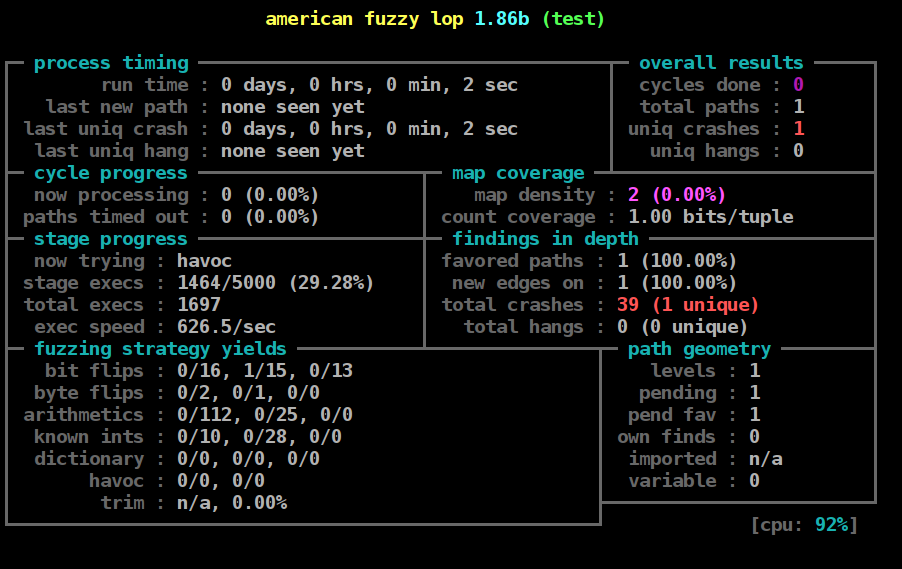
\includegraphics[width=0.9\linewidth]{images/American_fuzzy_lop's_afl-fuzz_running_on_a_test_program}
	\caption{AFL fuzzer}
	\label{fig:americanfuzzylopsafl-fuzzrunningonatestprogram}
\end{figure}

On the other hand, boofuzz is a Python-based fuzzing library most commonly used for protocol fuzzing. As such, it does not require code instrumentation to function. Instead, it supports building blueprints of protocols to be fuzzed using primitives and blocks. These can be thought of as representations of various common components of protocols, such as data types including strings, integers and bytes, but also other common features, such as length fields, delimiters and checksums. These allow users to specify protocol requests to be sent to the \ac{sut} and explicitly mark which portions of the request should be fuzzed via settings in the primitives. Possible settings on a per primitive/block level include the maximum length of data to be generated while fuzzing and also if the element in question should be fuzzed at all, or just be left at a default values. The option to define which parts of a protocol will be fuzzed at a field-by-field level gives boofuzz a high degree of flexibility. The exact fuzz data generated by the framework depends on the used blocks and settings, and then creates mutations based on the specified protocol structure. For example, a string primitive uses a list of many ``bad'' strings as a basis for mutation, which it then concatenates, repeats and otherwise mutates. Additionally, the \ac{sut} can be monitored for crashes and other unexpected behavior and the framework can furthermore be instructed to restart or reset the \ac{sut} when needed. In this paper, we use boofuzz primitives to generate our values for fuzzing, as detailed in Chapter \ref{chap:Fuzzing}.

\begin{figure}
	\centering
	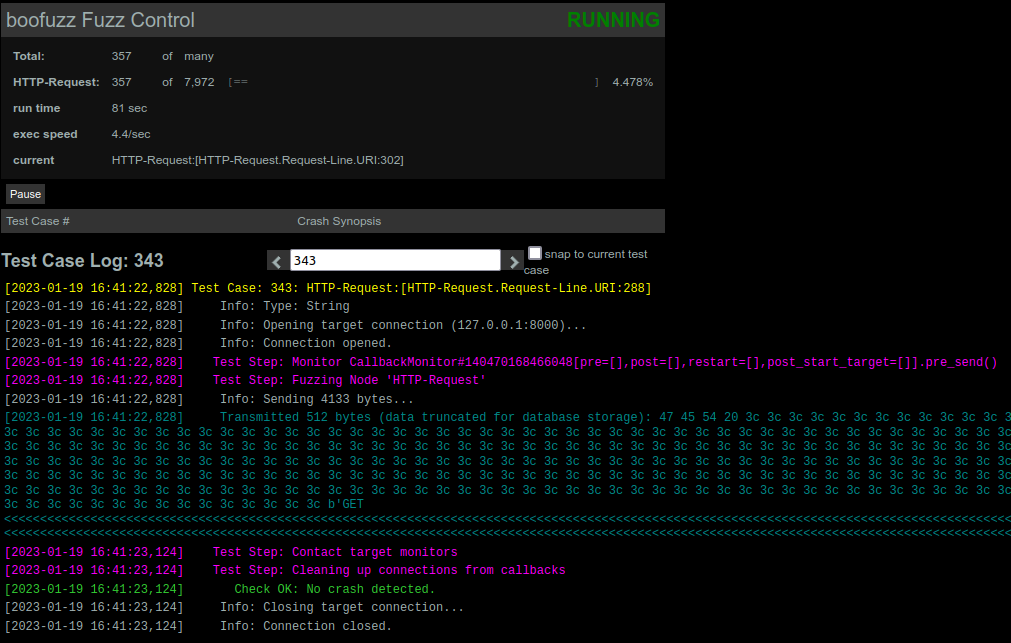
\includegraphics[width=0.9\linewidth]{images/boofuzz_control_center}
	\caption{Boofuzz fuzzer}
	\label{fig:boofuzzcontrolcenter}
\end{figure}

\newpage
\section{IPsec}
\ac{vpn}s are used to extend and or connect private networks across an insecure channel (usually the public internet). They can be used, e.g. to gain additional privacy from prying eyes such as Internet Server Providers, access to region-locked online content or secure remote access to company networks. Many different \ac{vpn} protocols exist, including PPTP, OpenVPN and Wireguard. Internet Protocol Security (\ac{ipsec}), is a \ac{vpn} layer 3 protocol suite used to securely communicate over an insecure channel. It is based on three sub-protocols, the \ac{ike} protocol, the \ac{ah} protocol and the \ac{esp} protocol. \ac{ike} is mainly used to handle authentication and to securely exchange as well as manage keys. Following a successful \ac{ike} round, either \ac{ah} or \ac{esp} is used to send packets securely between parties. The main difference between \ac{ah} and \ac{esp} is that \ac{ah} only ensures the integrity and authenticity of messages while \ac{esp} also ensures their confidentiality through encryption.

\begin{figure}[H]
\begin{centering}
	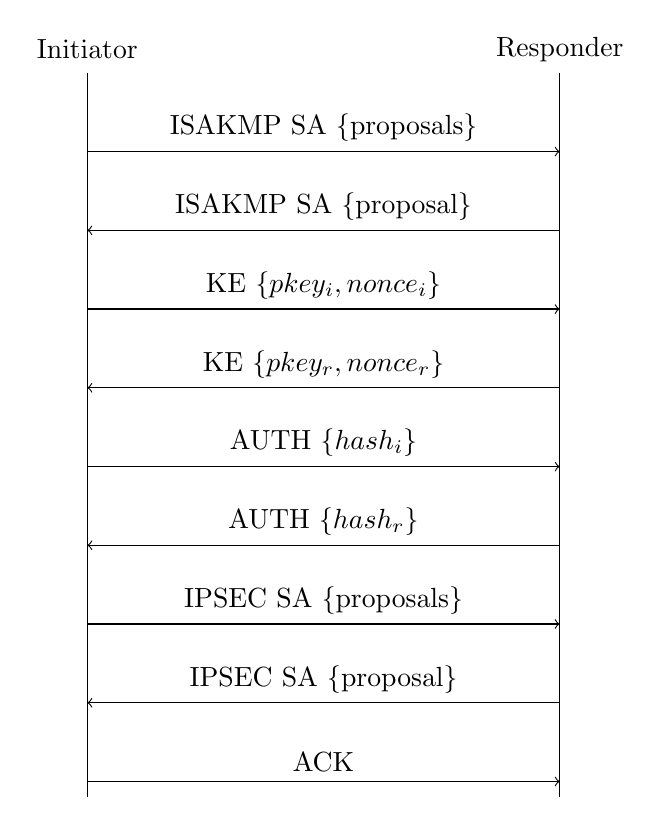
\begin{tikzpicture}[scale=1]
		\draw (-3,0) -- (-3,-9.2) (3,0) -- (3,-9.2);
		\node at (-3,.3) {Initiator};
		\node at (3,.3) {Responder};
		\draw[->] (-3,-1) -- node[midway,above] {ISAKMP SA \{proposals\}} (3,-1);
		\draw[<-] (-3,-2) -- node[midway,above] {ISAKMP SA \{proposal\}} (3,-2);
		\draw[->] (-3,-3) -- node[midway,above] {KE $\{pkey_i, nonce_i\}$} (3,-3);
		\draw[<-] (-3,-4) -- node[midway,above] {KE $\{pkey_r, nonce_r\}$} (3,-4);
		\draw[->] (-3,-5) -- node[midway,above] {AUTH $\{hash_i\}$} (3,-5);
		\draw[<-] (-3,-6) -- node[midway,above] {AUTH $\{hash_r\}$} (3,-6);
		\draw[->] (-3,-7) -- node[midway,above] {IPSEC SA \{proposals\}} (3,-7);
		\draw[<-] (-3,-8) -- node[midway,above] {IPSEC SA \{proposal\}} (3,-8);
		\draw[->] (-3,-9) -- node[midway,above] {ACK} (3,-9);
	\end{tikzpicture}
	\caption{IKEv1 between two parties}
	\label{fig:IKEv1}
\end{centering}
\end{figure}

The \ac{ike}v1 protocol works in two main phases, both relying on the \ac{isakmp}. Additionally, phase one can be configured to proceed in either Main Mode or Aggressive Mode. A typical exchange between two parties, an initiator (e.g. an employee connecting to a company network) and a responder (e.g. a company VPN server), using Main Mode for phase one and \ac{psk} authentication, can be seen in Figure \ref{fig:IKEv1}. In contrast, aggressive mode reduces the number of packets in phase one to only three. While faster, this method is considered to be less secure, as the authentication hashes are sent in clear text. In phase one (Main Mode), the initiator begins by sending a \ac{sa} to the responder. A \ac{sa} essentially details important security attributes required for a connection such as the encryption algorithm and key-size to use, as well as the authentication method and the used hashing algorithm. These options are bundled in containers called proposals, with each proposal describing a possible security configuration. While the initiator can send multiple proposals to give the responder more options to choose from, the responder must answer with only one proposal, provided both parties can agree upon one of the suggested proposals. This initial communication is denoted as \emph{ISAKMP SA} in Figure~\ref{fig:IKEv1} and also exchanges initiator/responder cookies, tokens used as identifiers for the remainder of the connection. Subsequently, the two parties perform a Diffie-Hellman key exchange, denoted as \emph{KE}, with the public key shorted to $pkey$, and send each other nonces used to generate a shared secret key \texttt{SKEYID} as detailed in Listing~\ref{lst:keying}. Here, \texttt{PSK} refers to the pre-shared key, \texttt{Ni/Nr} to the initiator/responder nonce and \texttt{CKY-I/CKY-R} to the initiator/responder identifier cookie. The symbol ``|'' is used to signify concatenation of bytes, not a logical or. Note that \ac{ike}v1 allows using various different authentication modes aside from PSK, including public key encryption and digital signatures. \texttt{SKEYID} is used as a seed key for all further session keys \texttt{SKEYID\_d}, \texttt{SKEYID\_a}, \texttt{SKEYID\_e}, with $g^{xy}$ referring to the previously calculated shared Diffie-Hellman secret and \texttt{prf} to a pseudo-random function (in our case, HMAC). 0, 1 and 2 are constants used to ensure that the resulting key material is different and unique for each type of key. Following a successful key exchange, all further messages of phase one and two are encrypted using a key derived from \texttt{SKEYID\_e} and \texttt{SKEYID\_a} for authentication. Note that the length of the actual encryption key depends on the used encryption algorithm, and is generated by concatenating hashes of \texttt{SKEYID\_e} and trimming the result until the desired length has been reached. This allows for the \texttt{SKEYID\_e} key to be used to generate arbitrary-length encryption keys. Finally, in the last section of phase one \emph{AUTH}, both parties exchange and verify hashes to confirm the key generation was successful. Once verification succeeds, a secure channel is created and used for phase two communication. If phase one uses Aggressive Mode, then only three packets are needed to reach phase two. While quicker, the downside of Aggressive Mode is that the communication of the hashed authentication material happens without encryption. This means, that using short \acp{psk} in combination with Aggressive Mode is inherently insecure, as the unencrypted hashes are vulnerable to brute-force attacks provided a short key-size~\footnote{\url{https://nvd.nist.gov/vuln/detail/CVE-2018-5389}}. The shorter phase two (Quick Mode) begins with another \ac{sa} exchange, labeled with \emph{IPSEC SA} in Figure~\ref{fig:IKEv1}. This time, however, the \ac{sa} describes the security parameters of the ensuing \ac{esp}/\ac{ah} communication and the data is sent authenticated and encrypted using the cryptographic material calculated in phase one. This is followed by a single acknowledge message, \emph{ACK}, from the initiator to confirm the agreed upon proposal. After the acknowledgment, all further communication is done via \ac{esp}/\ac{ah} packets, using \emph{SKEYID\_d} as keying material.

\begin{lstlisting}[float=ht, caption=IKE Keying, label=lst:keying]
	# For pre-shared keys: 
	SKEYID = prf(PSK, Ni_b | Nr_b)
	
	# to encrypt non-ISAKMP messages (ESP)
	SKEYID_d = prf(SKEYID, g^xy | CKY-I | CKY-R | 0)
	
	# to authenticate ISAKMP messages
	SKEYID_a = prf(SKEYID, SKEYID_d | g^xy | CKY-I | CKY-R | 1)
	
	# for further encryption of ISAKMP messages in phase two
	SKEYID_e = prf(SKEYID, SKEYID_a | g^xy | CKY-I | CKY-R | 2)
\end{lstlisting}

In addition to the packets shown in Figure~\ref{fig:IKEv1}, \ac{ike}v1 also specifies and uses so called \ac{isakmp} Informational Exchanges. Informational exchanges in \ac{ike}v1 are used to send \ac{isakmp} \emph{Notify} or \ac{isakmp} \emph{Delete} payloads. Following the key exchange in phase one, all Informational Exchanges are sent encrypted and authenticated. Prior, they are sent in plain. \ac{isakmp} \emph{Notify} payloads are used to transmit various error and success codes, as well as for keep-alive messages. \ac{isakmp} \emph{Delete} is used to inform the other communication partner, that a \ac{sa} has been deleted locally and request that they do the same, effectively closing a connection. 

Compared to other protocols, \ac{ipsec} offers a high degree of customizability, allowing it to be fitted for many use cases. However, in a cryptographic evaluation of the protocol, Ferguson and Schneier \textcite{ferguson1999cryptographic} criticize the complexity arising from the high degree of customizability as the biggest weakness of \ac{ipsec}. To address its main criticism, \ac{ipsec}-\ac{ike}v2 was introduced in RFC 7296 to replace \ac{ike}v1 \cite{kaufman2014internet}. Nevertheless, \ac{ipsec}-\ac{ike}v1 is still in wide-spread use to this day, with the largest router producer in Germany, AVM, still only supporting \ac{ike}v1 in their routers \cite{avm2022}. We use \ac{ipsec}-\ac{ike}v1 with Main Mode and \ac{esp} in this paper and focus on the \ac{ike} protocol as it is the most interesting from an AAL and security standpoint. % this part could maybe be moved to the introduction, not sure
